% Figure 5: Control Flow Collapse Comparison
\documentclass[tikz,border=10pt]{standalone}
\usepackage{tikz}
\usetikzlibrary{arrows.meta,positioning,shapes,calc,fit,backgrounds}

\begin{document}
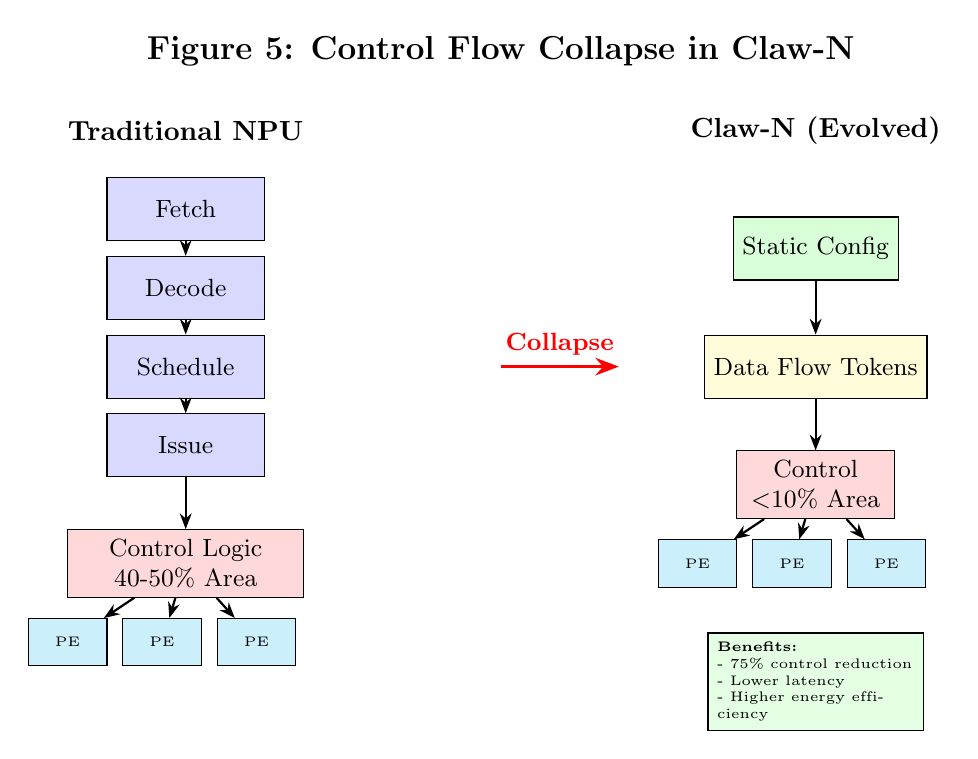
\begin{tikzpicture}[
    node distance=1cm,
    box/.style={rectangle, draw, minimum width=2cm, minimum height=0.8cm, align=center, font=\small},
    smallbox/.style={rectangle, draw, minimum width=1cm, minimum height=0.6cm, font=\tiny},
    arrow/.style={-{Stealth[length=2mm]}, thick}
]

% Title
\node[font=\large\bfseries] at (0,4) {Figure 5: Control Flow Collapse in Claw-N};

% Traditional NPU (left)
\node[font=\bfseries] at (-4,3) {Traditional NPU};

% Instruction fetch and decode
\node[box, fill=blue!15] (fetch) at (-4,2) {Fetch};
\node[box, fill=blue!15] (decode) at (-4,1) {Decode};
\node[box, fill=blue!15] (sched) at (-4,0) {Schedule};
\node[box, fill=blue!15] (issue) at (-4,-1) {Issue};

% Control logic overhead
\node[box, fill=red!15, minimum width=3cm] (control) at (-4,-2.5) {Control Logic\\40-50\% Area};

% PEs
\foreach \i in {0,1,2} {
    \node[smallbox, fill=cyan!20] (pe\i) at (-5.5+\i*1.2,-3.5) {PE};
}

\draw[arrow] (fetch) -- (decode);
\draw[arrow] (decode) -- (sched);
\draw[arrow] (sched) -- (issue);
\draw[arrow] (issue) -- (control);
\foreach \i in {0,1,2} {
    \draw[arrow] (control) -- (pe\i);
}

% Claw-N (right)
\node[font=\bfseries] at (4,3) {Claw-N (Evolved)};

% Data flow only
\node[box, fill=green!15] (config) at (4,1.5) {Static Config};
\node[box, fill=yellow!15] (tokens) at (4,0) {Data Flow Tokens};

% Minimal control
\node[box, fill=red!15, minimum width=2cm] (ctrl) at (4,-1.5) {Control\\$<$10\% Area};

% PEs with direct connection
\foreach \i in {0,1,2} {
    \node[smallbox, fill=cyan!20] (cpe\i) at (2.5+\i*1.2,-2.5) {PE};
}

\draw[arrow] (config) -- (tokens);
\draw[arrow] (tokens) -- (ctrl);
\foreach \i in {0,1,2} {
    \draw[arrow] (ctrl) -- (cpe\i);
}

% Benefit annotations
\node[draw, fill=green!10, align=left, font=\tiny, text width=2.5cm] at (4,-4) {
    \textbf{Benefits:}\\
    - 75\% control reduction\\
    - Lower latency\\
    - Higher energy efficiency
};

% Center arrow
\draw[very thick, -{Stealth}, red] (0,0) -- (1.5,0) node[midway, above, font=\small\bfseries] {Collapse};

\end{tikzpicture}
\end{document}
